\section*{\underline{PART D: Estimation}}
\markboth{PART D: Estimation}{}


\subsection*{Question 9: What is our best estimate of the true average repair time for the plant?}

In statistical analysis, the ``best estimate'' of a true, unknown population parameter (such as the true average repair time for all breakdowns across the entire plant) is the point estimate derived from a representative sample. Because our sample is drawn directly from the factory's historical Manufacturing Execution System (MES) records, it serves as an unbiased representation of the baseline operational environment. 

Therefore, our single best estimate is the sample mean ($\bar{x}$) of the pre-implementation baseline repair times. Based on our descriptive statistics calculations from Part B, our best point estimate for the true average repair time is \textbf{16.36 minutes}. Relying on the Law of Large Numbers, because our dataset captures an extensive history of stoppage events, we can be confident that this sample mean is a highly accurate proxy for the unknown true average.


\subsection*{Question 10: What range of values is reasonably plausible for the true population mean repair time?}

While the sample mean (16.36 minutes) is our best single-value estimate, we established in Part C that sample means are subject to sampling error and variability. Consequently, we cannot guarantee that our point estimate perfectly matches the exact true population mean. 

To account for this uncertainty and define a ``reasonably plausible range,'' we construct a 95\% Confidence Interval (CI) using the sample mean, standard deviation, and sample size.

Using the baseline dataset, we computed the following interval for the population mean:
\begin{itemize}
    \item \textbf{Lower Bound:} 14.63 minutes
    \item \textbf{Upper Bound:} 18.09 minutes
\end{itemize}

We can be 95\% confident that the true plant-wide average repair time falls within this specific range. Put simply, if we were to take 100 different downtime samples and compute CIs for each, approximately 95 would successfully contain the true average. 



\begin{figure}[H]
    \centering
    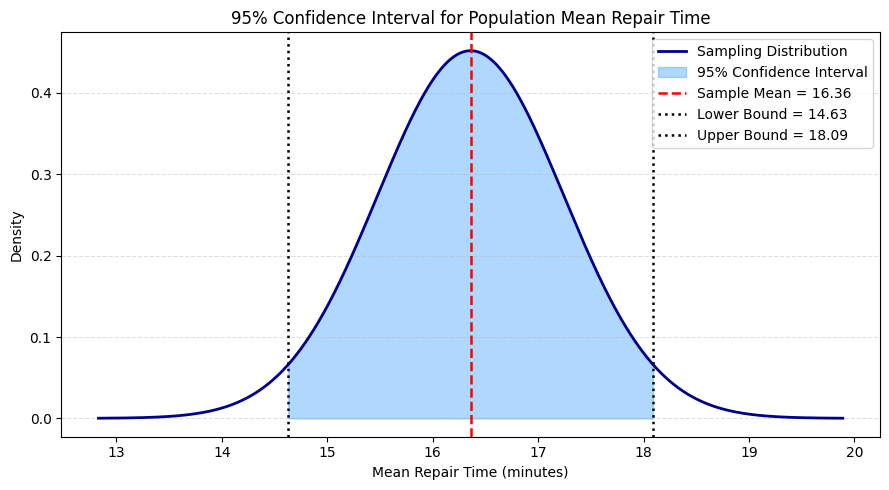
\includegraphics[width=0.85\linewidth]{figures/CI1.png}
    \caption{95\% Confidence Interval for the Population Mean Repair Time. The shaded region represents the plausible range [14.63, 18.09] minutes surrounding the point estimate of 16.36 minutes.}
    \label{fig:confidence_interval}
\end{figure}